\documentclass[11pt]{article}
\usepackage{hyperref}
\usepackage{amsthm}
\usepackage{amsmath}
\usepackage{amsfonts}
\usepackage{tikz}
\usepackage{ wasysym }
\usepackage{fancyvrb}

\newtheorem{example}{Example}


\author{Group 1:  Thalia Garmendez, Nicholas Jacob,\\ Harshkumar Parmar, Matt Scholelen}
\title{Homework 2 Advanced Analytics and Metaheuristics}

\begin{document}
\maketitle
%{\Large
%%Change Document name to: Graded Homework 1\_Jacob\_Nicholas
%\noindent NAME:  Nicholas Jacob\\ 
%STUDENT ID: \# 113578513\\
%HOMEWORK NUMBER: 1\\
%COURSE: DSA 5113 Advanced Analytics and Metaheuristics\\ 
%SECTION: ONLINE\\SEMESTER: Spring 2024\\
%INSTRUCTOR:  DR. Charles Nicholson\\
% SCORE:}
%
%\newpage
\begin{enumerate}
\item Grapes of Wrath
\begin{enumerate}
\item Grimes upper bound on grapes used for raisins.  We know that 25\% of the $8.4\times10^6$lb crop was ``A'' quality with the rest being ``B'' grade.  We also know that ``A grapes average 9 points per pound and ``B'' grapes average 5 points per pound.  Raisins require 8 points or higher in quality.  Here we end up with a small LP problem.  First we call $A$ the number of pounds of grade ``A'' grapes and $B$ the number of pounds of grade ``B''.  Our objective is to maximize the total pounds made into raisins:
\[
\text{maximize totalPounds: }A +B;
\]
We will have non-negative constraints on $A$ and $B$, as well as total production constraints
\[
A\leq 2 100 000\quad\text{ and }\quad B\leq 6 300 000
\]
Finally we have the quality constraint:
\[
\text{subject to qualityPoints: }9A +5B \geq 8\left(A+B\right)
\]
This one should get a small comment as we want the average number of points to be greater than 8 for our raisins.  We code this into our AMPL model and arrive at the following output.


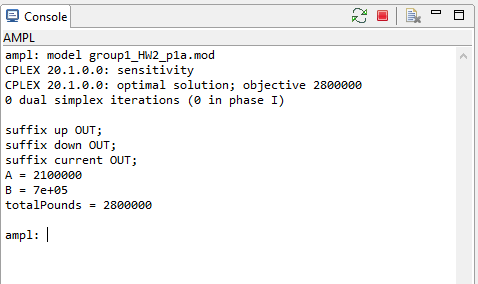
\includegraphics[width = .9\textwidth]{outputp1a.png}

Of course we could have done this with equality but this inequality method worked too.

\item To arrive at Bollman's assessment of the price of the grapes, it is important to consider the quality of the inputs.  We see that the entire lot was purchased for \$0.28 per pound but some of the grapes are clearly more valuable.  With the 25\% breakdown of type ``A'' to ``B'' we must account for that.  Moreover we must use the ratings to arrive at the appropriate value per pound of each type, ``A'' is rated 9 and ``B'' is rated 5, the higher the rating the more tha value to the company.  This creates a system of linear equations with $y$ begin price of type ``A'' and $z$ being price of ``B" in cents.  
\[
\left\{
\begin{array}{l}
2 100 000 y +6 300 000 z = 8 400 000 \times 28\\
\frac{y}{9} = \frac{z}{5}
\end{array}
\right.
\]
We solve this system with substitution and arrive at $y = 42$ and $z = 23\frac13$ prices reported are cents per pound.  Using these prices we see that jelly can be made entirely from the type ``B'' grapes and will require 19 pounds per product.  Therefore the grape cost for jelly is $19z = \$4.43\frac13$.  The analysis for the other two products is a bit more complicated.  Juice requires a 6 point average so if $a_j$ is the amount of high quality grapes and $b_j$ the amount of low quality grapes, we will need 
\[
9a_j+5b_j \geq 6(a_j+b_j)
\]
or
\[
3a \geq b.
\]
So for every 1 pound of high quality grapes, we can use at most 3 pounds of low quality grapes.  For purposes of computing the fruit cost, we will compute a minimum cost here but when the grapes are divided later, this price may change.  The computed minimum price for the juice grapes is
\[
15.5\frac{\left(y+3z\right)}{4} = \$4.34
\]
For the grapes, the minimum rating it 8 so
\[
9a_r+5b_r\geq 8(a_r+b_r)
\]
or
\[
a_r\geq 3b_r
\]
So each pound of low quality grapes we use in raisins, we must use at least 3 pound of high quality grapes.  We see then that the minimum price for the input grapes is \label{1b}
\[
6.75\frac{3y+z}4 = \$2.52.
\]
\item To formulate for AMPL, we ask for the decision variables to be the amount of each type of grape included in our raisins, jelly and juice.  We assume that the cost of the grapes is a fixed ratio based on quality scale points as outlined in \ref{1b} but not that the grape input should still be that fixed ratio when computing the price of our input grapes.  We consider overhead costs to be fixed and for the accounting department to figure out which product to allocate those costs to based on whatever they do in that department.

Our decision variables will be $(a_i,b_i)$ for $i\in\{raisins, juice, jelly\}$.  The objective is to maximize marginal profit (before accounting does their overhead magic).  We compute the number of products produced, $z_i$ as
\[
z_i = \frac{a_i+b_i}{poundsPerProduct_i}
\]
where $poundsPerProduct_i$ was given in the table.  The fruit cost will be computed as 
\[
fruitCost_i = 0.42a_i+0.233333b_i
\]
The our objective is
\[
\text{maximize: }\sum_{i}\left(sellingPrice_i-variableCost_i\right)\cdot z_i - fruitCost_i 
\]
We then have three constraints, quality, demand, and grape availability.  For quality, we get that
\[
9a_i+5b_i \geq quality_i(a_i+b_i).
\]
Demand constraint is
\[
z_i \leq maxDemand_i
\]
where the $maxDemand$ for raisins was set to infinity.  For grape availability, we had
\[
\sum_i a_i \leq 2 100 000\quad\text{and}\quad\sum_ib_i \leq 6 300 000.
\]
The AMPL solution seen below provides the following values;  
\begin{enumerate}
\item For raisin production was 408,148 whole units, juice was 8,709 whole units of juice, and 290,000 units of jelly.
\item For the maximized contribution to profit was \$1,306,120.
\item All grapes were utilized of both types as the slack of the $weightLimit$ was zero.
\item The average quality point count for the raisins, juice, and jelly were 8, 6, and 5 respectively as driven by the quality requirements.  We again see this in the slack of the constraint $qualityControl$.
\end{enumerate}

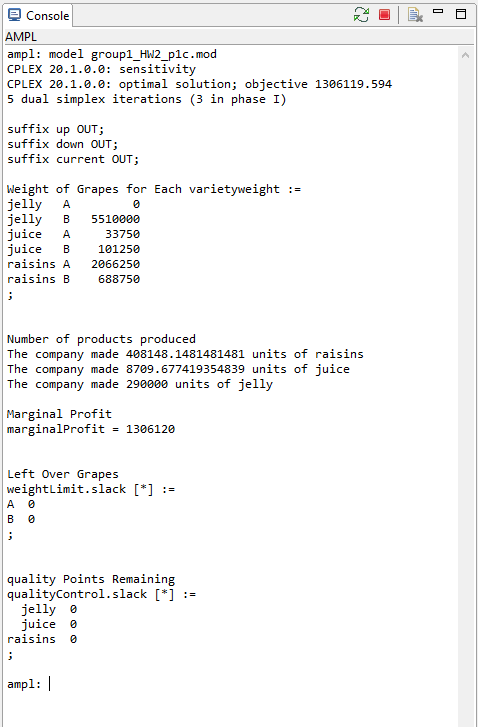
\includegraphics[width = .9\textwidth]{outputp1c.png} \label{1c}
\item To discover if we should purchase the additional grade $A$ grapes, we examine two differing solutions.  First we run the same model as \ref{1c} but include the shadow price of the constraint on the weightLimit.

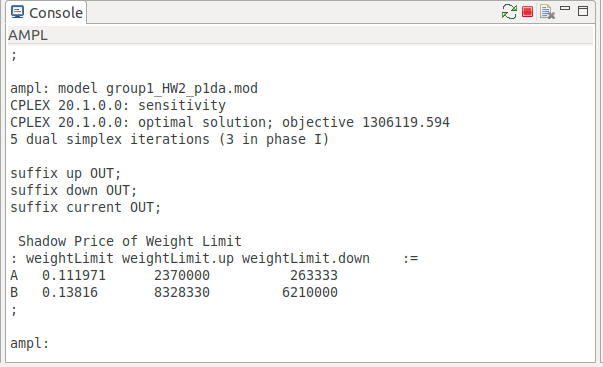
\includegraphics[width = .9\textwidth]{outputp1da.png}
\begin{enumerate}
\item Based on the shadow price from the above AMPL solution, for grade $A$ grapes, \$0.11 profit increase per pound of grade $A$ grapes, the purchase price of \$0.50 would provide \$0.03 profit per pound of increased amount of grade $A$ grapes.  The other reason to buy the extra grapes is that the shadow price upper limit would mean that the shadow price would be applicable to 270,000 lbs of the 300,000 lbs of extra grapes.  There would be a different shadow price above the limit, but it would only affect 30,000 lbs of the overall 300,000 lbs of extra grapes. 
\item Based on the original grade $A$ grape price of \$0.42 per pound and the shadow price, the maximum purchase price should only go to\$0.52, providing \$0.01 per pound of additional grade $A$ grape profit.  For grade $B$ grapes the maximum purchase price should only be \$0.35 per pound extra, because the original purchase price was \$0.23 per pound and the shadow price was \$0.13, which would still provide a \$0.01 of profit per pound of extra grade $B$ grape, up to roughly 2,000,000 additional grapes (based on the shadow price upper limit for grade $B$ grapes).

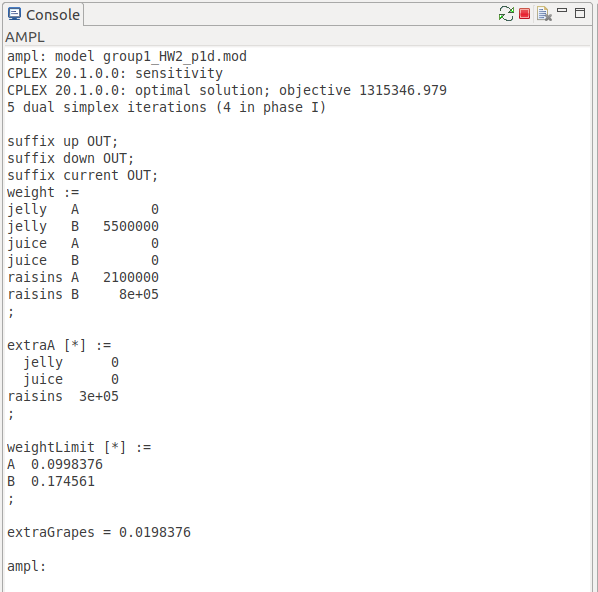
\includegraphics[width=.9\textwidth]{outputp1db.png}

\end{enumerate}
\item 
\begin{enumerate}
\item Mr Thomas forgot about the quality constraint and considered type $A$ and $B$ grapes to be the same cost.  We make only raisins in his model and make the largest marginal profit.  You would need for type $A$ or any type to be just slightly less than \$0.50 per pound to purchase.  His model results in \$473,436 more in profit than that found for part c.  The maximum price for extra grapes per pound should be no more that \$0.70 to maintain \$0.01 per pound profit increase, based on the shadow price for grapes, weightLimit value, seen in the AMPL output below. 

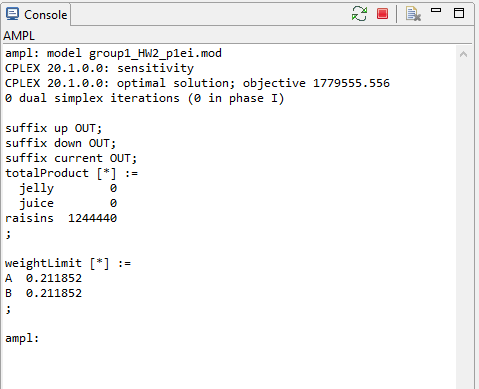
\includegraphics[width=.9\textwidth]{output1ei.png}
% completed edit to this point.
\item Based on Ms Bollman's profit figures, no raisins would be produced, with jelly production at 290,000 units and juice at 186,452 units.  The profit realized from this model would have been \$1,343,161, which is \$37,042 more than the profit realized in part c.  Based on Ms. Bollman's figures, the maximum amount to spend on extra grade $A$ grapes, would be \$0.54 to still have a \$0.01 per pound of extra grapes profit, from the weightLimit term in the AMPL output below. 

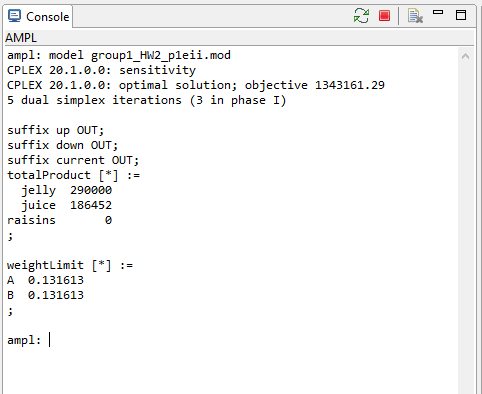
\includegraphics[width=.9\textwidth]{output1eii.png}

\item While both of our teammates report accurate results under their assumptions, they have forgotten important parts of our model.  Mr Thomas has ignored quality controls and assumed all grapes at the same price point.  Ms Bollman's analysis include accounting for grape quality but when she computes the marginal profit, she does not include the fact that juice made with higher quality grapes will in fact cost our company more.  In her analysis the whole price of the grapes our company paid for is not taken into account so the books will not balance later if we use her model.  Our model deals with all of these.  It also has a nice balance of products to keep our customers satisfied.  One limitation of our model is the lack of accounting of the overhead costs.  We are unclear if those should be attributed to each product in the way that Mr Thomas has done or if the accounting can be done in other ways to minimize our tax liability.
\end{enumerate}
\end{enumerate}
\item Titan's Dealings
\begin{enumerate}
\item To maximize Titan's return on the investment portfolio, we create our decision variable to be the amount invested in each Project, $amountInvested_a$.  We have a max amount that we are allowed to invest in each
\[
amountInvested_a \leq maxAmount_a.
\]
Then we have the trickiest part of this exercise, the investment constraint.  We start with \$1 000 000.  We use the cash-flow table presented in the email from Sharizi, $returns_{y,a}$ indexed on both year and project.  For 2021, we ask that the amount remaining, $amountNotInvested_y$,
\begin{align*}
amountNot&Invested_{2021} = 1 000 000\\
& + \displaystyle\sum_{a \in projects} amountInvested_a\cdot returns_{2021,a}\geq 0.
\end{align*}
This constraint requires that we can only invest up to our \$1 000 000.  We should not that all cash-flow in 2021 is negative as we are only investing in that year.  For the remaining three years, we have a similar function just without the initial cash but we allow for held over funds to gain interest
\begin{align*}
amountNot&Invested_y = 1.06 \cdot amountNotInvested_{y-1}\\
+&\displaystyle\sum_{a \in projects} amountInvested_a\cdot returns_{y,a}\geq 0.
\end{align*}
Some cash-flows are positive and some negative but we do not allow for borrowing of funds.  Lastly we succinctly state our objective
\[
\text{maximize: }amountNotInvested_{2024}
\]
This appears a bit odd as the objective but in year 2024, all returns will come back (no outflows) and this will give us the total returns of all investments.

Some assumptions made here is that there is a 6\% return on all funds held over from year to year.  No other opportunities for other projects present themselves.  All funds are withdrawn in 2024.  The cash-flow table is true and accurate.  Inflation will not degrade the value of our funds.  Here is our AMPL output:

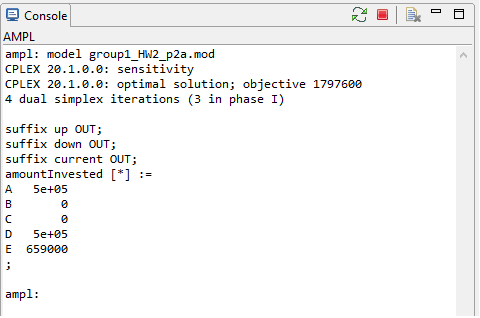
\includegraphics[width = .9\textwidth]{output2a.png}
\item There are two shadow prices within our model.  One associated with the constraint on the positivity of the $amountNotInvested$ and another on the $maxInvestments$.  Both are displayed in the output below.

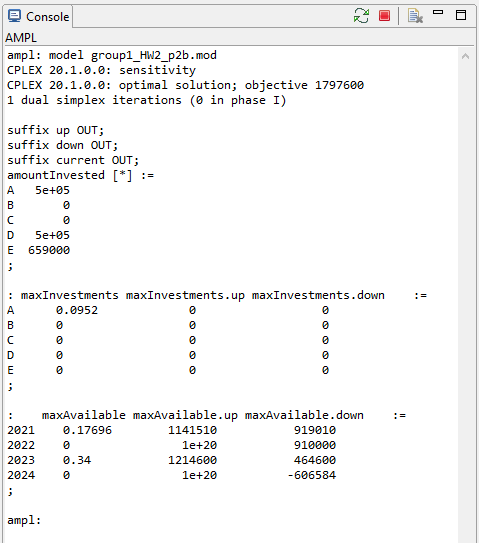
\includegraphics[width = .9\textwidth]{output2b.png}

We interpret the shadow price of $maxInvestments$ as the additional \$0.095 we would earn for every dollar more we could invest in project $A$.  So this is an additional way we could earn some more funds by moving that cap.  We do however note here that the availability of moving that cap up or down appears to be zero.  We think that is due to the fact that all the dollars were put elsewhere in the year that investment in $A$ was possible.  This shows that simply raising that investment cap will require other changes to the model.  

Next we examine the shadow price of the $maxAvailable$ variable.  The best way to think about this number would be potential gains we could derive by borrowing funds.  In the first year, we could earn 17 cents on any extra dollar included in the model.  We see that \$1 000 000 is in-between our up and down values.  This is because that was the amount we actually had to invest.  We see again there is excellent opportunity to borrow money in 2023 and increase our returns on projects.  We assume any funds borrowed in 2023 will be invested in project $E$ but the shadow price is slightly less than the actual rate of return on the investment $E$.  It would not be prudent to borrow to invest in any other years.  We speculate that these rates might be used as a hurdle rate in future years for evaluating any new project.


\item We explore several ways to examine this question.  First we will look at the opportunity cost for each of our decision variables.  This output is presented below by using .current method.

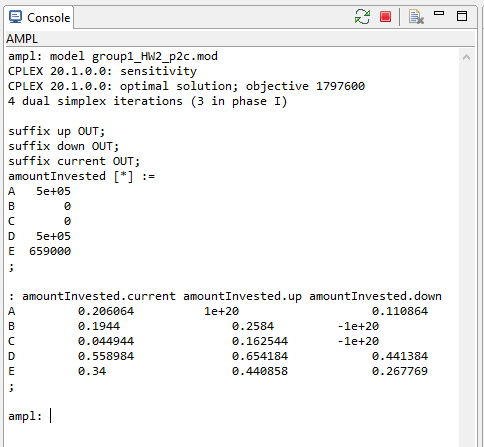
\includegraphics[width = .9\textwidth]{output2c.png}

These values can be interpreted as the slope of the optimal solution associated with each of these values.  We note that we only invest in the 3 highest slopes as we maximize our return.  We suspect that there is room to change the returns on project $D$ and $E$ as we can see in the up and down values.  We are uncertain about the actual values that we might be able to change returns to based on this output without some more knowledge of this method.

We will next examine $E$ and $D$ at the new payout rates by looking at the hurdle rate of 10\%.  These are 
\[
NPV_E = -1+\frac{1.34}{1.1} = 0.218
\]
and
\[
NPV_D = -1+\frac{1.7}{1.1^3} = 0.277.
\]
With both of these $NPV$s, we have no better investment so we suspect that we will continue to contribute to these funds.

Next we consider the $IRR$ for completeness.  To find the $IRR$, we must solve the following equations
\[
0 = -1+\frac{1.34}{1+r}
\]
and 
\[
0 = -1 +\frac{1.7}{(1+r)^3}.
\]

Thus we get that $IRR_E = 34\%$ and $IRR_D = 19.5\%$.  These both will still be our two highest $IRR$ rates for our company.

Lastly, we go ahead and change the data file to see what might happen with these new rates of return.  What we observe is that yes we do indeed continue investing into each account in the same fashion but our overall return does drop a bit.

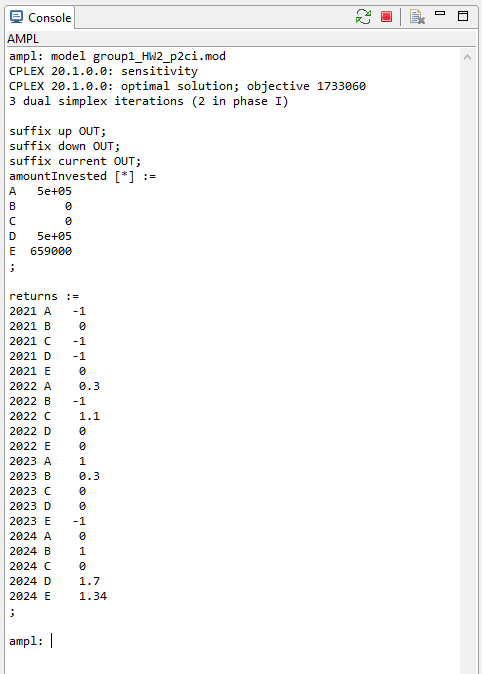
\includegraphics[width = .9\textwidth]{output2ci.png}



\item Let's look at the NPV's and IRR's of each of these investments.  We see the NPV's (with the hurdle rate at 10\%) as follows
\[
NPV_F = -1+\frac{0.8}{1.1} +\frac{0.45}{1.1^2} = 0.099
\]
and
\[
NPV_G = -1 +\frac{1.1}{1.1} +\frac{0.15}{1.1^3} = 0.112
\]
We can also compute the IRR's by setting the NPV to zero and solving for the rate $r$.  For investment $F$
\[
0 = -1 +\frac{0.8}{1+r} +\frac{0.45}{(1+r)^2} = -1 +\frac{1.25+0.8r}{(1+r)^2}
\]
Simplifying to the quadratic equation
\[
r^2+1.2r-0.25 = 0
\]
So 
\[
r_F = \frac{-1.2\pm\sqrt{1.2^2-4\cdot(-0.25)}}{2} = 18.1\%
\]
of course we ignore the negative value.  We follow a similar process needing to solve the equation
\[
0 = -1 +\frac{1.1}{1+r} +\frac{0.15}{(1+r)^3}.
\]
Arrives at 
\[
0 =r^3+1.9r^2+0.8r-0.25
\]
( \href{https://www.calculatorsoup.com/calculators/algebra/cubicequation.php?a=1\&b=1.9\&c=.8\&d=-.25\&action=solve}{but solved a cubic}) and arrive at
\[
r_G = 20.4\%
\]

We believe we would utilize project $F$ since it does slightly better than $A$ but not use $G$ as it ties up the funds the entire time and does worse than $D$.

\item Adding $F$ into the model we arrive at


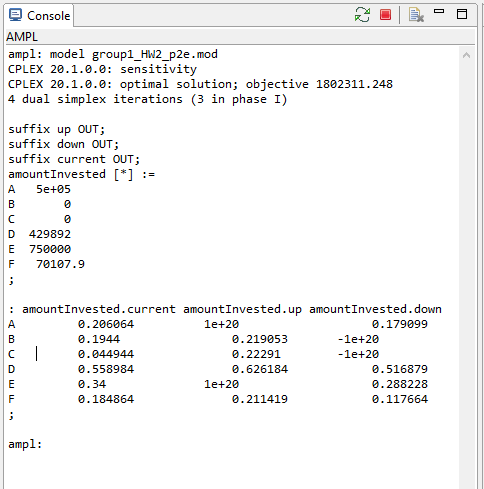
\includegraphics[width = .9\textwidth]{output2e.png}

We see that some of the moneys that had been invested in fund $D$ in the first year are now instead invested into $F$ but it is honestly a small pittance.  This increases our profitability slightly.  


Moneys invested in $F$ will also be invested in $E$ so perhaps some compounding allows for this to be more profitable than just sticking with $D$.  The small decrease in $D$ would suggest that its $IRR$ will fall below that of $F$ so at that point we would most likely invest more into $F$.  We do not think a small tweak on $E$ will change its usage in the model.  We see this in the opportunity analysis and the ability to move that slope downward.  We also note that $E$ allows for funds put into $A$ and $F$ get reinvested in a timely manner.  We see this as a strength for $E$ in our model.
\end{enumerate}
\end{enumerate}



\end{document}
